\section{Estado del arte y antecedentes}

\subsection{Estado del arte del problema a tratar} \label{sec_estado_arte_problema}

El problema de la estimación de la edad a partir de restos óseos ya se ha tratado en distintas ocasiones, desde modificaciones a la propuesta de Todd, propuestas de como automatizar la estimación utilizando las características que proponía Todd, hasta estudios que utilizaban técnicas de visión por computador para recoger y procesar las características de los restos.

En 1990, J. M. Suchey y S. Brooks propusieron una modificación a la propuesta de Todd \cite{sucheyBrooks}, en la que evaluaban $739$ restos óseos y llegaban a la conclusión de que era posible reducir las diez fases propuestas por Todd a seis fases, modificando el criterio de cada una de las fases y añadiendo cierto error marginal, aunque con un $95\%$ de confianza con los nuevos intervalos propuestos. Esta modificación es una de las más aceptadas por la comunidad científica, aunque la mayor parte de trabajos siguen utilizando las fases propuestas por Todd.

% TODO buscar estado del arte enfocado a clasificación a sistemas basados en reglas

Uno de los más relevantes es un estudio publicado en el año 2015 en la revista \textit{Journal of forensic sciences} \cite{modelandoHuesos3D}, en el que se escaneaban los restos tomados como muestras para la variación de la sínfisis púbica y con esta variación realizar la estimación de la edad utilizando un modelo de regresión lineal y las seis fases propuestas por Suchey y Brooks. El conjunto de datos utilizado en este experimento se compone de $41$ esqueletos de personas estadounidenses y logran obtener una raíz del error cuadrático medio de unos $17.15$ años.

\begin{figure}[H]
	\centering
	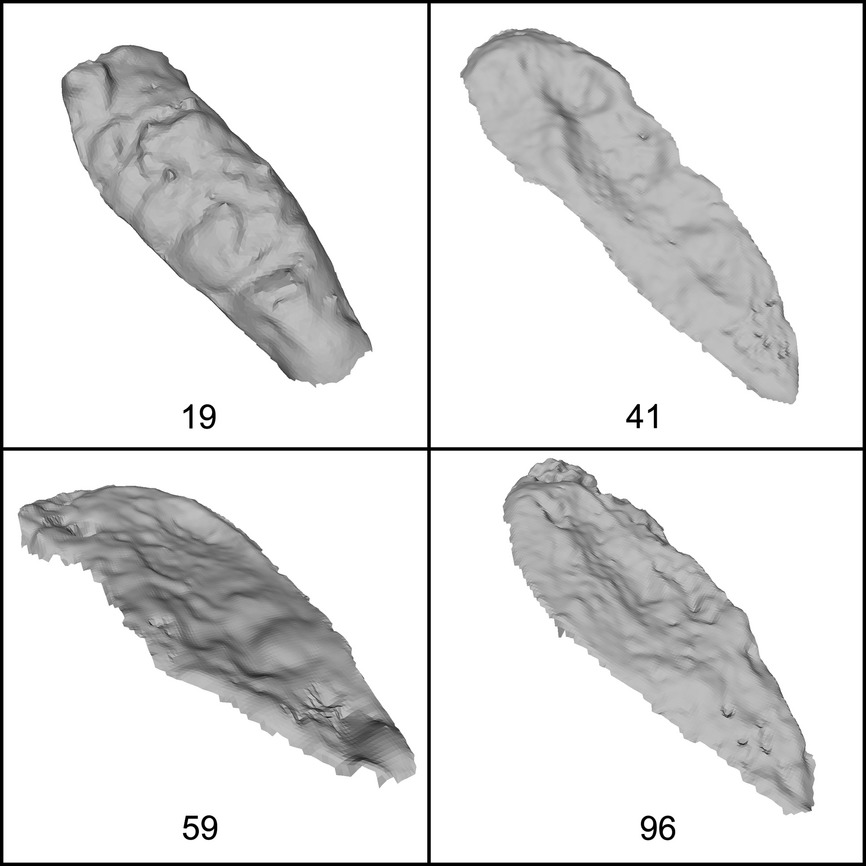
\includegraphics[scale = 0.4]{escaneo_huesos.jpg}
	\caption{Visualización del escaneo de la sínfisis púbica en cuatro individuos. La edad de la muerte aparece en la parte inferior de cada imagen. Imagen obtenida de \cite{modelandoHuesos3D}.}
	\label{fig:escaneo_huesos}
\end{figure}

Ese mismo año, los mismos autores presentaron una mejora \cite{mejoraModelandoHuesos3D} en la que, en lugar de utilizar la variación total de la sínfisis púbica, utilizaban la flexión de un plano de forma que dicho plano coincida con la superficie del hueso. De esta forma, utilizando un conjunto de datos similar a su experimento anterior y la curvatura de la sínfisis púbica entrenaron un modelo de regresión lineal con el que obtuvieron una raíz del error cuadrático medio de unos $19$ años.

A finales de 2015, Beatrix Dudzik y Natalie R. Langley, de la Universidad de Tennessee y la Universidad Lincoln Memorial, propusieron \cite{componentBased} varios modelos basados en árboles de decisión y regresión logística multinomial. Para estos experimentos utilizaron 5 características de la sínfisis púbica de 47 individuos de entre 18 y 40 años. Obtuvieron muy buenos resultados, con una tasa de acierto del $94\%$ aunque solo utilizaban 3 de las 6 fases propuestas por Suchey y Brooks.

\begin{figure}[H]
	\centering
	\begin{subfigure}{.5\textwidth}
	  \centering
	  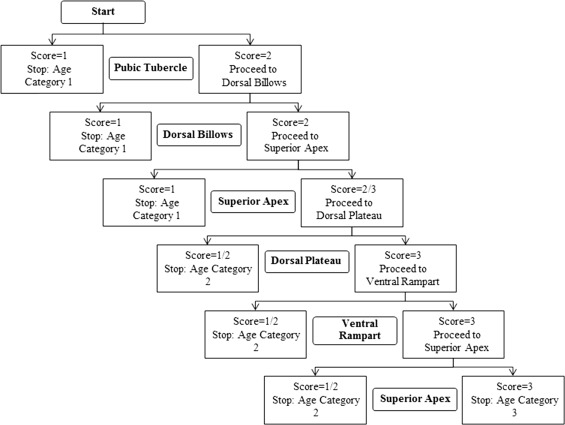
\includegraphics[scale = 0.7]{cita_7_arbol.jpg}
	  \caption{Árbol de decisión implementado en \cite{componentBased}}
	  \label{fig:arbol_c7}
	\end{subfigure}%
	\begin{subfigure}{.5\textwidth}
	  \centering
	  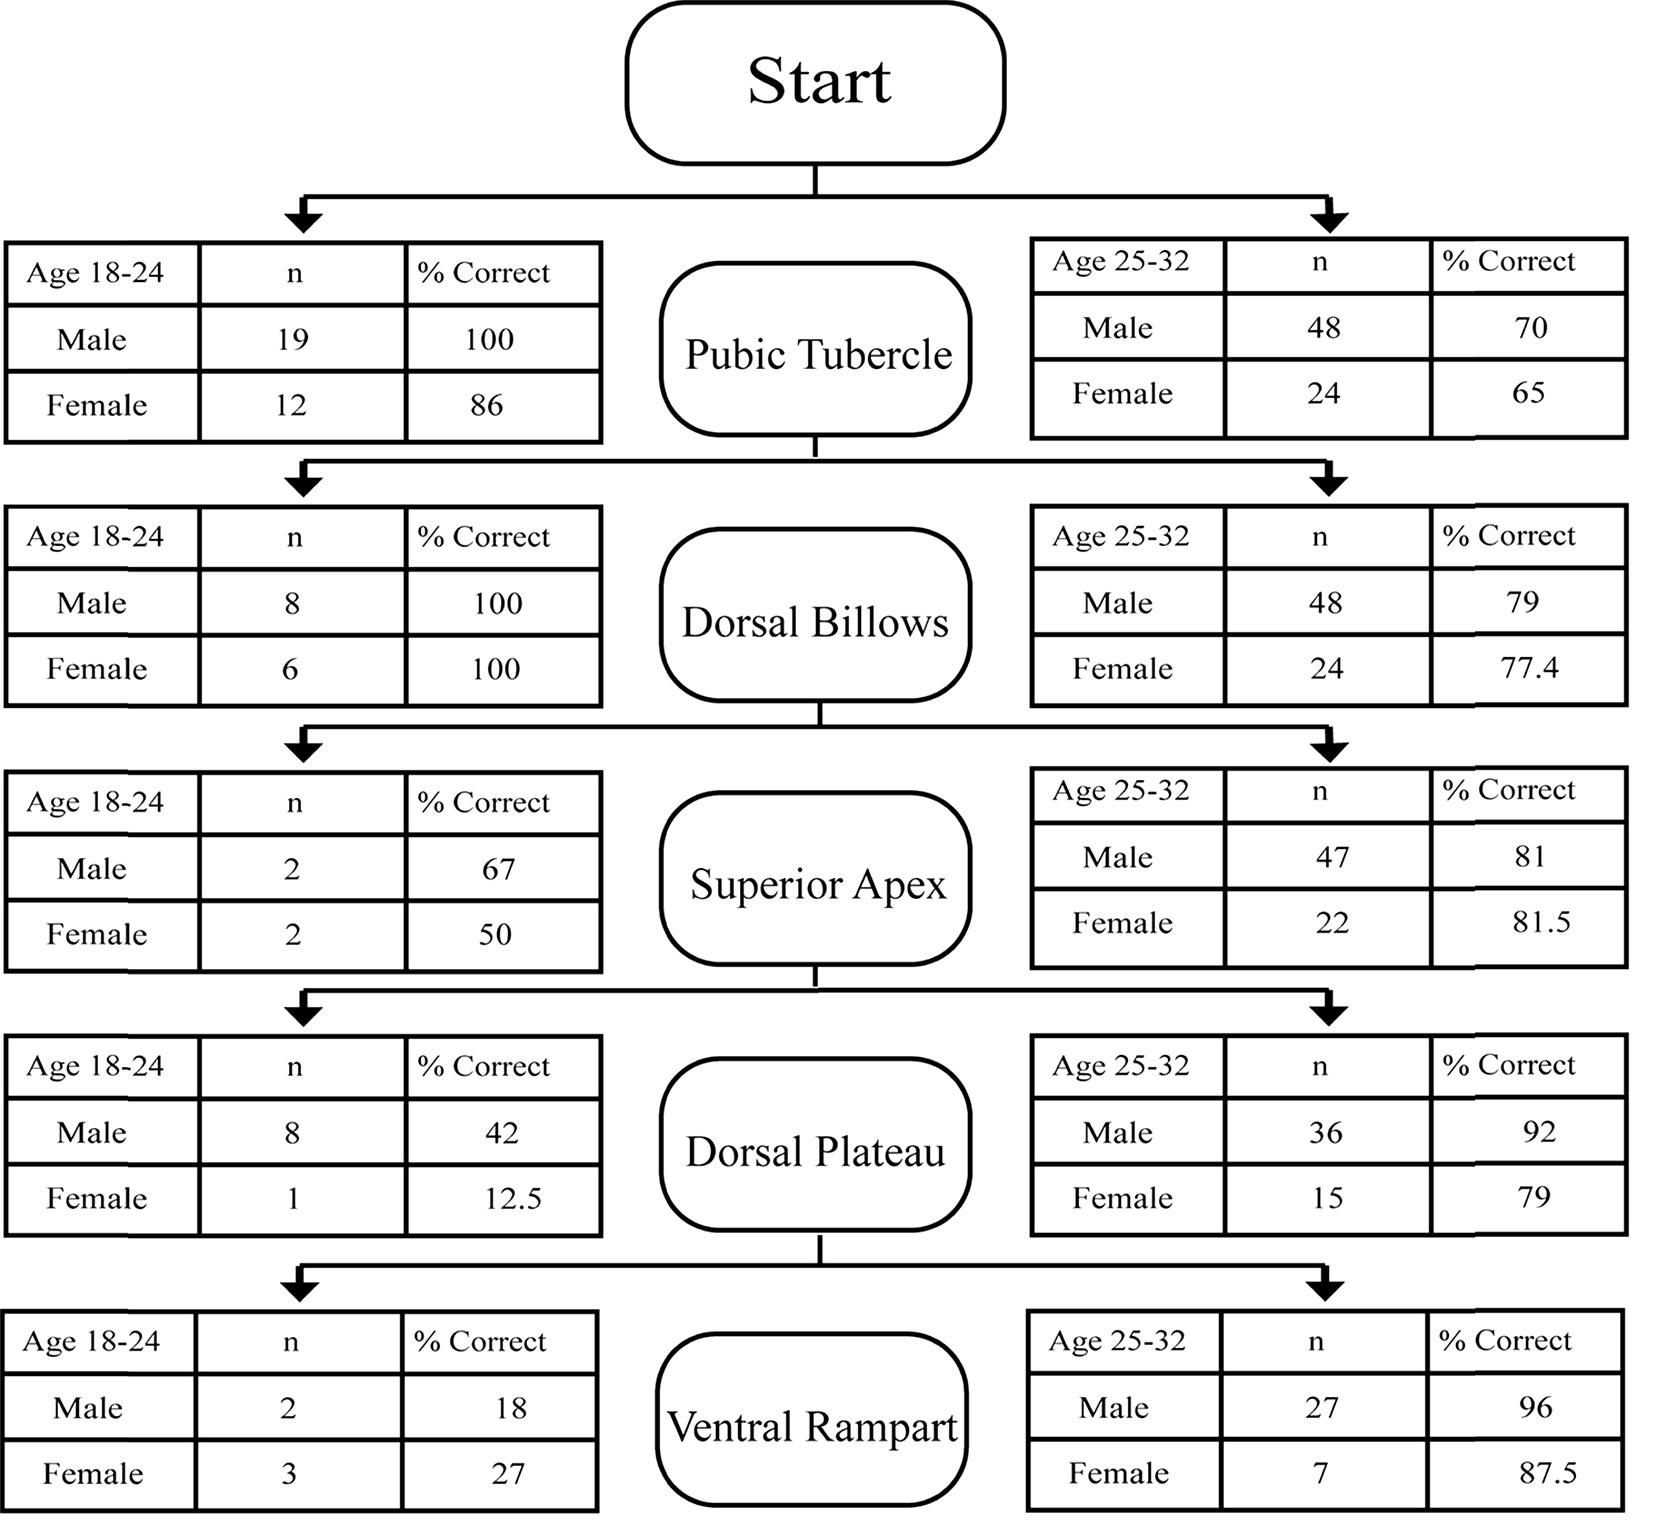
\includegraphics[scale = 0.8]{cita_7_ejemplo_dos_fases.jpg}
	  \caption{Porcentaje de acierto para la fase 1 y 2 de \cite{componentBased}.}
	  \label{fig:acierto_cita7}
	\end{subfigure}
	\caption{Imágenes obtenidas de \cite{componentBased}.}
	\label{fig:arboles_cita7}
\end{figure}



Más adelante, en 2018, varios investigadores de la República Checa publicaron un trabajo \cite{estimacionHuesosCadera} en el que, con un conjunto de $941$ restos óseos de personas de distinta raza entre 19 y 100 años, utilizando datos de los huesos de la cadera estudiaban las características comunes y las que diferenciaban las distintas edades, y consideraban 9 modelos distintos para realizar una estimación, desde un sistema de puntuación tradicional, utilizando la variación entre los huesos, distintos de regresión lineal, árboles de decisiones o redes neuronales artificiales. De estos modelos se llega a la conclusión que el mejor es un modelo de regresión multinomial, con el que obtienen una raíz del error cuadrático medio de unos $12.5$ años.

En 2017 investigadores de la Universidad de Granada publicaron un artículo preliminar de cara a obtener un modelo descriptivo basado en reglas con el que realizar la estimación de la edad a partir de la sínfisis púbica \cite{fuzzyAgeEstimation}. Utilizando $74$ muestras clasificadas manualmente consiguen entre 17 y 20 reglas utilizando árboles de decisión difusos que consiguen un error absoluto medio de $1.68$ años, aunque el resultado no es totalmente fiable debido a que no consiguen reglas para algunas fases propuestas por Todd.

Más adelante, en 2021, este mismo equipo con la ayuda de investigadores de la Universidad de Cordoba publicaron una continuación de su estudio \cite{NSLVOrdAge}. En este caso, utilizando el mismo conjunto de datos que utilizaremos nosotros, aplicando técnicas de balanceo y sobremuestreo de datos para resolver problemas relativos a dicho conjunto de datos, han enfocado el problema como un problema de clasificación ordinal. Utilizando el software NSLVOrd \cite{NSLVOrd}, un algoritmo de clasificación ordinal basado en el enfoque de aprendizaje de reglas de forma iterativa publicado por investigadores de la Universidad de Granada en 2016, son capaces de obtener una raíz del error cuadrático medio de $12.34$ años utilizando 34 reglas para las distintas fases. Este es, hasta este momento, el mejor resultado del estado del arte de este problema, y además en este estudio se discute sobre la importancia de las características a observar en la sínfisis púbica propuestas por Todd, llegando a la conclusión de que ciertas características nunca se utilizan, y por lo tanto no entran en juego a la hora de realizar la estimación de la edad.


% Comentar el enfoque de Gilbert y McKern y diferenciar ambos enfoques

Otro enfoque de este problema es el propuesto por McKern y Stewart en el año 1957 \cite{primeraPropuestaMcKern} y que luego ampliarían en 1973 junto a Gilbert \cite{propuestaGilbert}. En lugar de resolver el problema con un enfoque de clasificación, proponían un método en el que se le asignan valores numéricos a cada uno de los distintos posibles estados de cada característica observada en la sínfisis púbica, y con esos valores conseguir una fórmula que estimase la edad. En este trabajo utilizaremos este enfoque de cara a tratar este problema como un problema de regresión. En la siguiente sección haremos una presentación más detallada de este método.

Uno de los primeros trabajos que aplico este enfoque fue un estudio de la Universidad de Tokio \cite{primerTrabajoGilbert}. Los autores utilizan una extensión de la regresión lineal, regresión lineal múltiple, ya que utilizan siete características de la sínfisis púbica y una constante de cara a obtener fórmula que les sea capaz de estimar la edad. Tras los distintos experimentos, consiguen obtener unos resultados bastante buenos aunque, como los propios autores indican, el rango de edades con el que se ha trabajado es bastante limitado, siendo solo entre 18 y 38 años y solo contando con 135 muestras de sínfisis púbica.

Años más tarde, en 1995, Investigadores del departamento de Medicina Forense del All India Institute of Medical Sciences en Nueva Delhi, India, utilizarán este trabajo para aplicarlo a 41 individuos de entre doce y setenta y cinco años, comparando los resultados utilizando regresión lineal múltiple con el sistema de clasificación de Todd \cite{estudioComparandoGilbertTodd}. En este trabajo se logran obtener resultados significativamente mejores que con la propuesta de Todd, además de sumarse a las conclusiones de otros trabajos, que aunque tomen un enfoque distinto, se podrían modificar las fases propuestas por Todd, ya que se observan como algunas de las variables tienden a zonas entre dos fases de Todd, además de encontrar algunas de las características de la sínfisis púbica irrelevantes a la hora de estimar la edad en muchas de las fases.



\subsection{Sistemas basados en reglas}



\subsection{Programación Genética}

La Programación Genética apareció como una adaptación de los algoritmos evolutivos para representar programas de ordenador como cromosomas en una estructura de árbol. A pesar de que su aparición fue en 1985 no fue hasta principios de 1990 cuando este método comenzó a ser más utilizado gracias a John Koza \cite{kozaGP}.

La forma en la que la Programación Genética expresa los cromosomas permite resolver problemas de distintos tipos dando soluciones sencillas de interpretar, por este motivo este algoritmo y sus variaciones han sido bastante utilizadas.

Uno de los primeros trabajos fue de publicado por P. A. Whigham en 1995 \cite{PGgramaticas}, en el que se utiliza una gramática inicial libre del contexto para generar expresiones a utilizar en el algoritmo, y que durante el entrenamiento el algoritmo complete la gramática y la amplíe con nuevas reglas, siendo un claro ejemplo de aprendizaje incremental.

Tras demostrar la potencia de Programación Genética para aprender estructuras gramaticales, una de sus principales aplicaciones fue sistemas basados en reglas, donde se utilizaban algoritmos evolutivos para aprender las reglas del sistema.

En 1996, Edward Tunstel, investigador de la NASA y Mo Jamshidi, investigador de la Universidad de Nuevo México, publicaron un artículo \cite{PGcontrolRobots} en el que utilizaban sistemas basados en reglas difusas para un sistema de control de un robot en un entorno tridimensional, donde se utilizaba Programación Genética para el aprendizaje de las reglas del sistema, aprovechando la estructura de gramática de los individuos de la población. Utilizando tan solo poblaciones de entre diez y veinte reglas, escogiendo la regla con mejor ajuste, y con doce ejecuciones del algoritmo, obtuvieron doce reglas capaces de resolver el problema.

\begin{figure}[H]
	\centering
	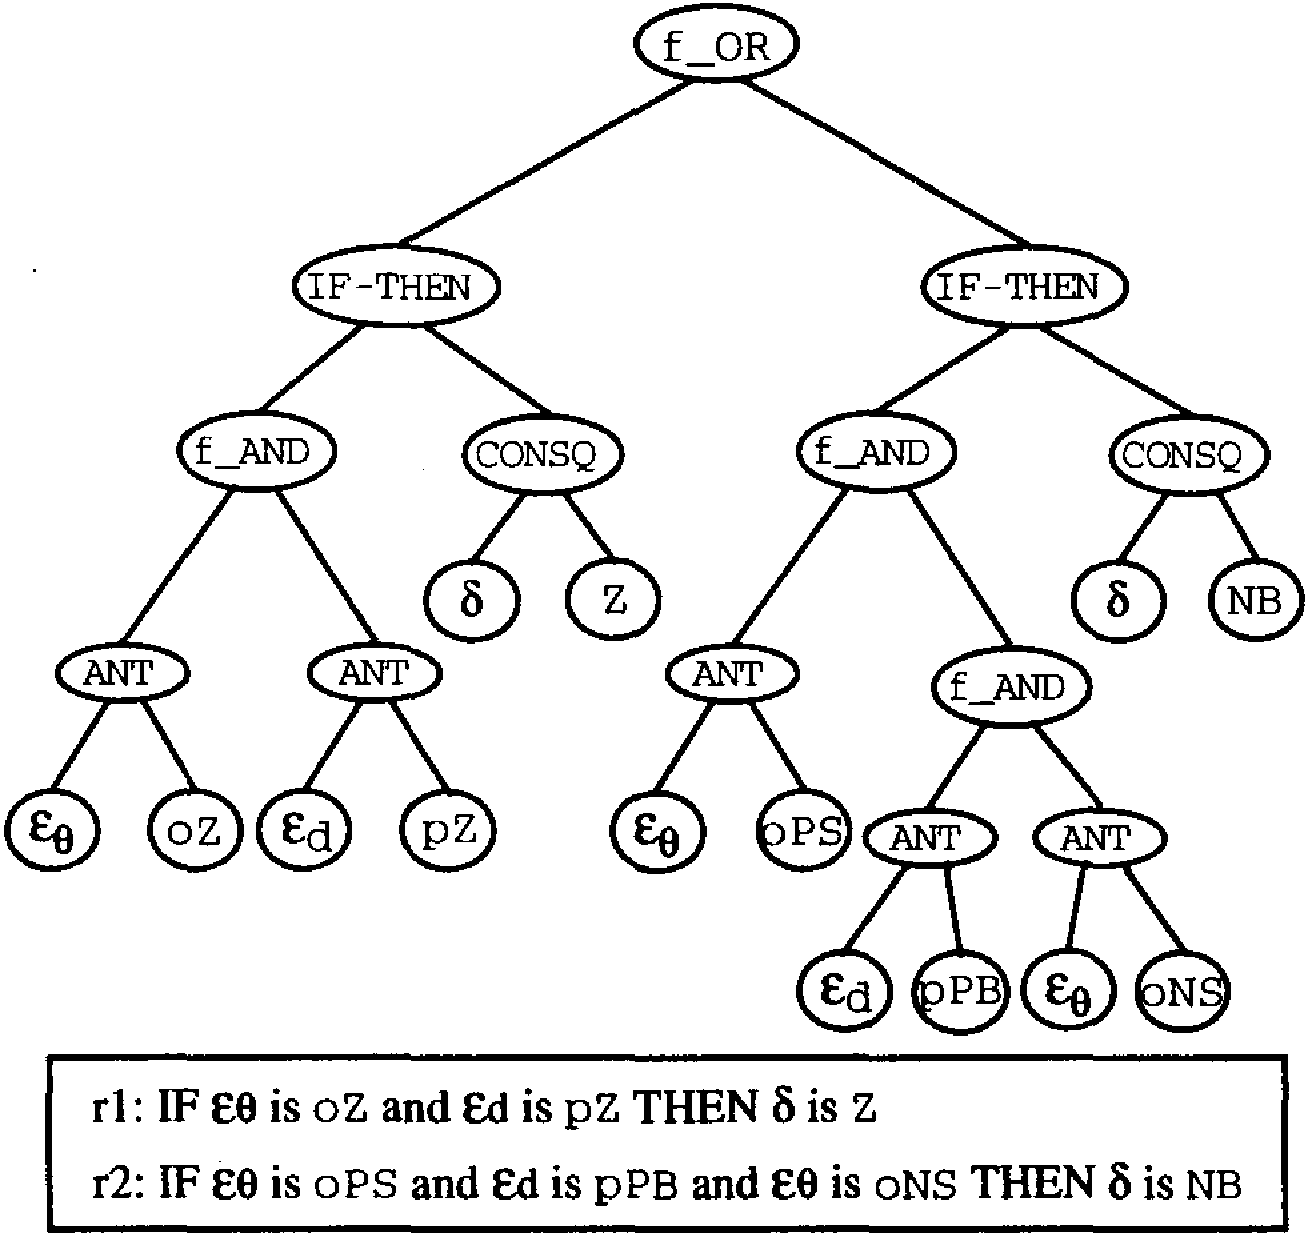
\includegraphics[width = 0.5\textwidth]{imagenes_papers/imagen_arbol_regla_robots.png}
	\caption{Ejemplo de regla difusa representada como un árbol del trabajo \cite{PGcontrolRobots}.}
	\label{fig:imagen_arbol_regla_robots}
\end{figure}

Más adelante, en el año 2000, investigadores del Centro Federal de Educación Tecnológica de Paraná, en Brasil, desarrollaron un trabajo \cite{trabajoChestPain} bastante similar al problema propuesto debido a la alta cantidad de clases y las pocas observaciones del problema disponibles. En este trabajo proponen un sistema basado en reglas de cara a predecir diagnósticos de doce tipos distintos de dolor torácico. De cara a obtener las reglas necesarias utilizan Programación Genética, lanzando para cada clase diez ejecuciones del algoritmo, manteniendo la mejor regla para cada clase como resultado, obteniendo un total de doce reglas. A pesar del bajo número de observaciones, consiguen unos resultados muy altos tanto de sensibilidad (probabilidad de detectar los verdaderos positivos) como de especificidad (probabilidad de detectar los verdaderos negativos), además de una simplicidad de las reglas (valor obtenido a partir del número máximo de nodos y el número de nodos de cada regla) muy cercanos a uno, mostrando la clara ventaja de sistemas basados en reglas para obtener modelos explicables.

También en el año 2000, investigadores de la Universidad de Oviedo proponen \cite{GAPnichosFuzzyRules} ciertas mejoras a GA-P, una modificación de Programación Genética que se mencionará más adelante, de cara a aprender un sistema basado en reglas difusas. Proponen utilizar GA-P para aprender tanto las reglas que conformarán el sistema como las particiones difusas de las características del conjunto de datos. En este trabajo también se discute la importancia de que los operadores de cruce y de mutación conserven la forma de la gramática propuesta de cara a no generar reglas inválidas, cruzando tan solo los subárboles de mismo tipo en la forma BNF donde se define la gramática.

Otro trabajo interesante es el publicado por Tsakonas et al en 2004 \cite{reglasDosDominiosMedicosComparacion} donde se proponen evaluar la potencia de Propagación Genética en dos problemas médicos, así como comparar los resultados con otros métodos como árboles C4.5. Para el primer problema se obtienen resultados con alrededor de un 70\% de acierto utilizando C4.5, utilizando Programación Genética para regresión simbólica se consigue un acierto cercano al 90\%, mientras que con Programación Genética obteniendo un sistema basado en reglas se consigue un acierto algo superior al 85\%. Para el segundo problema C4.5 consigue un acierto del 70\%, mientras que Programación Genética consigue alrededor de un 98\% con las distintas variantes.

En 2005 investigadores de la Universidad de Córdoba publican un trabajo \cite{grammarBasedPG} en el que utilizan una modificación de Programación Genética para utilizar el algoritmo en base a una gramática, de forma que los operadores de cruce y mutación respeten esa gramática generando siempre reglas válidas. En este trabajo también se compara este método con otros métodos como árboles de decisión o inducción de reglas, así como dos formas de interpretar el conjunto de reglas con una instancia:

\begin{enumerate}
	\item Se evalúan las reglas de forma secuencial, y la primera regla encontrada en la que se cumple todo el antecedente, se le asigna la clase del consecuente a dicha instancia.
	\item Se evalúan todas las reglas, contando el número de reglas satisfechas por cada clase. La clase con el mayor número de reglas satisfechas será la clase escogida para la instancia.
\end{enumerate}

Además, en este trabajo, en lugar de obtener distintas reglas lanzando varias veces el algoritmo, un individuo de la población representará un conjunto completo de reglas, con la restricción de que existe al menos una regla para cada clase, de forma que en este trabajo se entrenan conjuntos completos, no reglas por separado. Finalmente vemos como la propuesta es muy competitiva con respecto a otros algoritmos como ID3 o C4.5, consiguiendo valores muy similares de acierto en distintos conjuntos de datos.

En el año 2007 investigadores de la Universidad de Kassel, en Alemania, proponen \cite{mejorasPGreglas} ciertas mejoras al algoritmo de Programación Genética para obtener mejores resultados al aprender reglas. En este trabajo se discute el problema de Programación Genética de la dependencia de los distintos individuos de la población. De cara a resolver este problema proponen cambiar la representación de las reglas, binarizando los distintos símbolos, operadores, acciones y componentes que conforman la gramática y representando las reglas con forma de vector de ceros y unos, aunque contará con distintas secciones de ceros y unos que representarán las distintas partes de la regla. De esta forma son capaces de aplicar Programación Genética utilizando los operadores de un algoritmo genético simple. Aunque con esta modificación se obtienen resultados con reglas muy complejas y bastante sobreajuste, este trabajo nos puede ayudar a ver distintas propuestas sobre el algoritmo original que podrían modificar el funcionamiento del sistema si fuese necesario.

Otro de sus principales usos es regresión simbólica, ya que nos ofrece un algoritmo muy bueno para problemas en los que los resultados son variables, no se conoce a priori la forma que tendrá el resultado, además de todas las ventajas de los algoritmos evolutivos.

La principal forma de conseguir que Programación Genética trabaje con regresión simbólica es modificar los cromosomas propuestos por John Koza, en lugar de ser programas de ordenador, generador por gramáticas, los cromosomas serán expresiones matemáticas, manteniendo siempre la forma de árbol. Esta modificación es tan simple por reemplazar la gramática por una gramática que genere expresiones matemáticas, con los operadores que se estimen oportunos.

En 1995, investigadores de la Universidad de Georgia publicaban un artículo \cite{primerGAP} en el que proponían utilizar Programación Genética para hacer regresión simbólica, es decir, aprender una fórmula matemática estructurada como un árbol. En este trabajo se mencionan los principales problemas de la Programación Genética para regresión simbólica, todos ellos derivados de que este algoritmo solo puede modificar la estructura de las expresiones, no su contenido como tal, no siendo capaz de trabajar con valores numéricos constantes, además de generar ramificaciones complejas para obtener cierta constante. En este trabajo se propone añadir un algoritmo genético a Programación Genética de cara a resolver estos problemas aprendiendo las constantes numéricas en un cromosoma independiente, de ahí el nombre GA-P (Genetic Algorithm-Programming).

Más adelante esta variación de Programación Genética se utilizará en diversos trabajos, como el publicado por investigadores de la Universidad de Oviedo y la Universidad de Granada en 1999 \cite{GAPredElectrica}, donde utilizando este algoritmo consiguen unos resultados bastante buenos en dos problemas reales aplicando regresión simbólica, el trabajo del año 2000 de los investigadores del Laboratorio Nacional de Computación Científica de Brasil, donde publican un artículo \cite{PGregresionSimbolica} donde explican y proponen en detalle los distintos operadores necesarios para GA-P, así como otro trabajo del año 2000 en el que investigadores de la Universidad de Granada utilizan GA-P para aprender consultas booleanas \cite{GAPFormulasBooleanas} en el que demuestran la versatilidad del algoritmo para distintos problemas además de obtener soluciones fácilmente interpretables.



\newpage
